\باب{برقی اور میکانی توانائی کا باہمی تبادلہ}
برقی رو یا مقناطیسی بہاو کی مدد سے برقی توانائی کو میکانی توانائی یا میکانی توانائی کو برقی توانائی میں تبدیل کیا جاتا ہے۔ مختلف مشین میں یہ عمل ہوتا ہے۔ ناپنے کے مشین نہایت کم طاقت کا تبادلہ کرتے ہیں۔ ان میں لاؤڈ سپیکر، مائکروفون وغیرہ شامل ہیں۔ ان کے برعکس ایک اور قسم کے مشین قوت پیدا کرتے ہیں۔ ان میں برقی مقناطیس، رِیلے\فرہنگ{رِیلے}\حاشیہب{relay}\فرہنگ{relay}  وغیرہ شامل ہیں۔ ایک تیسری قسم، جن میں برقی موٹر اور جنریٹر شامل ہیں، لگاتار توانائی کو ایک شکل سے دوسری شکل میں تبدیل کرتے ہیں۔

اس باب میں مقناطیسی بہاو کی مدد سے توانائی کے تبادلہ پر غور کیا جائے گا۔برقی رو کی مدد سے توانائی کے تبادلہ کو انہیں طرح کے طریقوں سے حل کیا جاتا ہے اگرچہ ان کا تذکرہ اس کتاب میں نہیں کیا جائے گا۔

 اس باب میں جو تراکیب ہم سیکھیں گے وہ بہت اہمیت رکھتے ہیں اور انجنیئرنگ میں بہت سے مسائل حل کرنے میں مدد گار ثابت ہوتے ہیں۔

\حصہ{مقناطیسی نظام میں قوت  اور  قوت مروڑ}
اگر ایک برقی میدان میں برقی بار \عددیء{q} رکھا جائے تو اس پر قوت
\begin{align}
\kvec{F}=q \kvec{E}
\end{align}
پائی جاتی ہے۔اگر برقی بار مثبت ہو تو یہ قوت برقی شدت \سمتیہ{E} کی سمت میں ہوتی ہے اور اگر برقی بار منفی ہو تو یہ قوت \سمتیہ{E} کی الٹ سمت میں ہوتی ہے۔ اسی طرح اگر ایک برقی بار مقناطیسی میدان میں حرکت کر رہا ہو اور اس کی \اصطلاح{سمتی رفتار}\فرہنگ{سمتی رفتار}\حاشیہب{velocity} \سمتیہ{v} ہو تو اس پر قوت
\begin{align}\label{مساوات_برقی_میکانی_تبادلہ_مقناطیسی}
\kvec{F}=q \left(\kvec{v} \times \kvec{B} \right)
\end{align}
پائی جاتی ہے۔ اس مرتبہ مثبت برقی بار پر قوت کی سمت \اصطلاح{دائیں ہاتھ کے قانون}\حاشیہب{right hand rule} سے معلوم کی جاتی ہے۔ اگر دائیں ہاتھ کی چار انگلیاں \سمتیہ{v} کی سمت میں رکھ کر انہیں \سمتیہ{B} کی سمت میں موڑا جائے تو انگوٹھا \سمتیہ{F} کی سمت میں ہو گا۔ منفی برقی بار پر قوت اس کے مخالف سمت میں ہو گی۔یہاں سمتی رفتار \عددیء{q} اور \سمتیہ{B} کے مابین ہے۔ اگر ایک برقی بار بیک وقت مقناطیسی اور برقی میدان میں حرکت کر رہا ہو تب اس پر قوت ہمیں گزشتہ دو قوانین ملا کر یعنی مساوات \اصطلاح{لورینز}\فرہنگ{مساوات لورینز}\حاشیہب{Lorenz equation}\فرہنگ{Lorenz equation}  سے ملتی ہے۔
\begin{align}
\kvec{F}=q \left(\kvec{E}+\kvec{v} \times \kvec{B}  \right)
\end{align}
مساوات  \حوالہ{مساوات_برقی_میکانی_تبادلہ_مقناطیسی} میں اگر \عددیء{\kvec{v}=\dif \kvec{L} / \dif t} لی جائے تو اسے یوں لکھا جا سکتا ہے۔
\begin{gather}
\begin{aligned}
\kvec{F}&=q \left(\frac{\dif \kvec{L}}{\dif t} \times \kvec{B} \right)\\
&=\frac{q}{\dif t} \left(\dif \kvec{L} \times \kvec{B} \right)\\
&=i \left(\dif \kvec{L} \times \kvec{B}  \right)
\end{aligned}
\end{gather}
%
\ابتدا{مثال}
شکل \حوالہ{شکل_تبادلہ_طاقت_لچھے_پر_قوت_اور_مروڑ} میں ایک لچھا مقناطیسی میدان میں دکھایا گیا ہے۔لچھے کی رداس \عددیء{15} سم، محوری لمبائی \عددیء{50} سم اور اس میں برقی رو  \عددیء{5} ایمپیئر ہے۔کثافتِ مقناطیسی بہاو کو نقطہ دار نوک والی لکیروں سے شمالی قطب سے جنوبی قطب کی جانب دکھایا گیا ہے۔اگر کثافتِ مقناطیسی بہاو \عددیء{0.55} ٹیسلہ ہو تو 
\begin{itemize}
\item
لچھے کے اطراف پر قوت معلوم کریں اور
\item
لچھے پر قوت مروڑ \سمتیہ{\tau} معلوم کریں
\end{itemize}
%
\begin{figure}
\centering
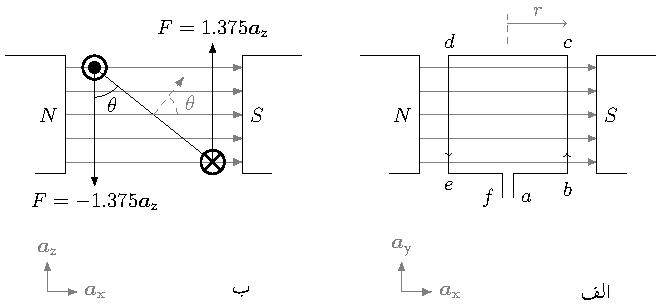
\includegraphics{figEnergyConversionTorqueOnOneTurn}
\caption{ایک چکر کے لچھے پر قوت اور قوت مروڑ}
\label{شکل_تبادلہ_طاقت_لچھے_پر_قوت_اور_مروڑ}
\end{figure}
%
حل:
	شکل-الف اور ب میں کارتیسی اکائی سمتیہ دیئے گئے ہیں۔اگر برقی تار کے سروں کو نظر انداز کیا جائے اور اسے ایک بند دائرہ سمجھا جائے تو  شکل-الف میں  برقی رو کی سمت میں تار کے اطراف کی لمبائیاں 
\begin{align*}
\kvec{L}_{bc}&=l \ay\\
\kvec{L}_{cd}&=-2 r \ax\\
\kvec{L}_{de}&=-l \ay\\
\kvec{L}_{eb}&=2 r \ax
\end{align*}
ہیں جبکہ \عددیء{\kvec{B}=B_0 \ax} ہے۔یوں مساوات \حوالہ{مساوات_برقی_میکانی_تبادلہ_مقناطیسی}  سے ان اطراف پر قوت
\begin{align*}
\kvec{F}_{bc}&= i \left(\kvec{L}_{bc} \times B_0 \ax \right)\\
&=5 \left(0.5 \ay \times 0.55 \ax \right)\\
&=-1.375 \az\\
\kvec{F}_{cd}&= 5\left(-0.3\ax \times 0.55 \ax \right)\\
&=0\\
\kvec{F}_{de}&= 5 \left(-0.5\ay \times 0.55 \ax \right)\\
&=1.375 \az\\
\kvec{F}_{ea}&= 0
\end{align*}
نیوٹن ہو گی۔ہم دیکھتے ہیں کہ قوت محوری لمبائی کی جانب اطراف پر ہی لاگو  ہے۔یہ دو قوت حصہ با میں دکھائے گئے ہیں جہاں سے یہ واضح ہے کہ یہ قوت مروڑ پیدا کریں گی۔ اس قوت مروڑ کی سمت دائیں ہاتھ کے قانون سے بھی با آسانی معلوم کی جا سکتی ہے۔قوت مروڑ
\begin{align*}
\kvec{\tau}&=-1.375 \times 2 \times 0.15 \times \sin \theta \ay\\
&=-0.4125 \sin \theta \ay
\end{align*}
نیوٹن-میٹر ہے۔
\انتہا{مثال}
%
	 ان مساوات کا استعمال صرف سادہ ترین جگہوں ممکن ہوتا ہے۔ استعمال میں آنے والی مشین میں ان مساوات سے قوت کا تعین کرنا نہایت مشکل ثابت ہوتا ہے۔ اب ہم وہ طریقہ سیکھتے ہیں جس کی مدد سے ہم مختلف مشین میں قوت کا تعین کر سکیں گے۔ اس طریقہ کو توانائی کا طریقہ کہتے ہیں اور یہ توانائی کے اٹل ہونے پر مبنی ہے۔

گھومتی برقی مشین میں عموماً دو لچھے ہوتے ہیں۔ ان میں ایک لچھا  مشین کے ساکن حصہ پہ لپٹا ہوتا ہے اور اسی لئے ساکن رہتا ہے۔ لہٰذا  اس کو \اصطلاح{ساکن لچھا}\فرہنگ{ساکن لچھا}\فرہنگ{لچھا! ساکن}\حاشیہب{stator coil}\فرہنگ{stator coil}   کہتے ہیں ۔  دوسرا لچھا  مشین کے گھومنے والے حصہ پہ لپٹا ہوتا ہے اور مشین گھومنے سے یہ بھی گھومتا ہے۔ لہٰذا اس کو \اصطلاح{گھومتا لچھا}\فرہنگ{گھومتا لچھا}\فرہنگ{لچھا!گھومتا}\حاشیہب{rotor coil}\فرہنگ{rotor coli}  کہتے ہیں۔  ایسے مشین  کو اس طرح سمجھنا نہایت آسان ہے کہ ہم ان دو لچھوں کو دو مقناطیس سمجھیں۔ جس طرح دو مقناطیس اگر قریب لائے جائیں تو یہ کوشش کرتے ہیں کہ ایک کا شمال \عددیء{N} دوسرے کے جنوب \عددیء{S} کی سمت  ہو۔

 موٹر میں دونوں  لچھے مقناطیس پیدا کرتے ہیں۔ ساکن لچھے کا مقناطیسی بہاو،  گھومتے لچھے کے مقناطیسی بہاو سے کچھ آگے رہتا ہے اور  اسے کھینچتا رہتا ہے۔ ایسا کرنے سے یہ کام کرتا ہے۔ جنریٹر میں اس کے برعکس  گھومتا لچھا، ساکن لچھے پر کام کرتے ہوئے اس میں برقی دباو پیدا کرتا ہے۔

توانائی کے طریقے کو شکل \حوالہ{شکل_تبادلہ_توانائی_نظام_بطور_ڈبہ}  کی مدد سے سمجھا جا سکتا ہے۔یہاں مقناطیسی نظام کو ایک ڈبہ کی شکل میں دکھایا گیا ہے۔ اس کو برقی توانائی مہیا کی جاتی ہے جس سے یہ میکانی توانائی پیدا کرتا ہے۔ یہاں برقی توانائی کے دو متغیرہ  \عددیء{e} اور \عددیء{i} ہیں اور میکانی توانائی کے متغیرہ فاصلہ \عددیء{x} اور میدانی قوت\حاشیہد{میدانی قوت \عددیء{F_m} میں چھوٹی لکھائیی میں \عددیء{m} لفظ میدانی کو ظاہر کر رہا ہے۔} \عددیء{F_m} ہیں۔ اس شکل میں بائیں جانب یعنی ابتدائی یا اولین جانب \عددیء{i} کا رُخ باہر سے اندر کی طرف ہے اور دائیں جانب یعنی ثانوی جانب \عددیء{F_m} کا رُخ اندر سے  باہر کی جانب ہے۔یہ  ٹرانسفارمر دور کے شکل \حوالہ{شکل_ٹرانسفارمر_کامل_بار_بردار_ٹرانسفارمر}  کی مانند ہے۔

اگر نظام میں توانائی کی ضیاع کو توانائی کے ذخیرہ ہونے سے علیحدہ کرنا ممکن ہو تو ایسی صورت میں توانائی کے ضیاع  کو بیرونی رکن سے پیش کیا جاتا ہے۔ شکل \حوالہ{شکل_تبادلہ_توانائی_قوت_پیدا_کرتا_آلا}   میں ایک ایسا ہی نظام دکھایا گیا ہے جس میں  لچھا برقی نظام کو پیش کرتا ہے اور حرکت کرنے والا حصہ میکانی نظام کو پیش کرتا ہے۔ یہاں لچھے میں توانائی کے ضیاع کو، بیرونی  مزاحمت \عددیء{R} سے ظاہر کیا گیا ہے۔
\begin{figure}
\centering
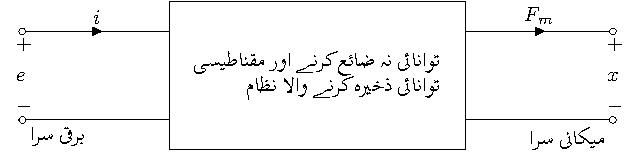
\includegraphics{figEnergyConversionBasicBlockDiagram}
\caption{ برقی توانائی سے میکانی توانائی کے تبادلہ کا نظام۔}
\label{شکل_تبادلہ_توانائی_نظام_بطور_ڈبہ}
\end{figure}
%
\begin{figure}
\centering
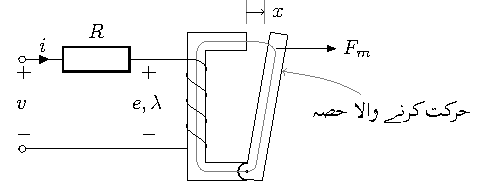
\includegraphics{figEnergyConversionForceGeneratingDevice}
\caption{ قوت پیدا کرنے والا آلا۔}
\label{شکل_تبادلہ_توانائی_قوت_پیدا_کرتا_آلا}
\end{figure}

توانائی کا بنیادی اصول کہتا ہے کہ توانائی نا تو پیدا کی جا سکتی ہے اور نا ہی اسے تباہ کیا جا سکتا ہے۔ اس کو صرف ایک قسم  سے دوسرے قسم کی توانائی میں تبدیل کیا جا سکتا ہے۔ لہٰذا اسے جو برقی توانائی \عددیء{\partial W_{\textup{برقی}}} دی جائے  اس میں سے کچھ میکانی توانائی \عددیء{\partial W_{\textup{میکانی}}}  میں تبدیل ہو گی، کچھ  مقناطیسی میدان میں  ذخیرہ ہو گی یعنی \عددیء{\partial W_{\textup{مقناطیسی}}} اور بقایا مختلف طریقوں سے  ضائع \عددیء{\partial W_{\textup{ضائع}}} ہو گی  جو ہمارے کسی کام نہ آ سکے گی۔ یعنی
\begin{align}
\partial W_{\textup{برقی}}=\partial W_{\textup{میکانی}}+\partial W_{\textup{مقناطیسی}}+\partial W_{\textup{ضائع}}
\end{align}
اگر برقی توانائی کے ضیاع کو نظرانداز کیا جائے تو
\begin{align}
\partial W_{\textup{برقی}}=\partial W_{\textup{میکانی}}+\partial W_{\textup{مقناطیسی}}
\end{align}
اس مساوات کو \عددیء{\partial t} سے تقسیم کرنے سے حاصل ہوتا ہے

\begin{align}
\frac{\partial W_{\textup{برقی}}}{\partial t}=\frac{\partial W_{\textup{میکانی}}}{\partial t}+\frac{\partial W_{\textup{مقناطیسی}}}{\partial t}
\end{align}
یہ مساوات توانائی کی بجائے طاقت کی بات کرتا ہے۔ اگر ہم بائیں ہاتھ کی جانب یعنی برقی طاقت کو \عددیء{e i} لکھیں اور  دائیں ہاتھ کی جانب   میکانی حصہ میں \عددیء{\partial W_{\textup{میکانی}}=F_m \partial x} لکھیں تو
\begin{align}
e i = F_m \frac{\partial x}{\partial t} +\frac{\partial W_m}{\partial t}
\end{align}
حاصل ہوتا ہے جہاں \عددیء{W_{\textup{مقناطیسی}}}  کو \عددیء{W_m} لکھا گیا ہے۔مساوات \حوالہ{مساوات_مقناطیسی_دور_فیراڈے_قانون}   کے استعمال سے اسے یوں لکھا جا سکتا ہے۔
\begin{align}
i \frac{\partial \lambda}{\partial t}=F_m \frac{\partial x}{\partial t}+\frac{\partial W_m}{\partial t}
\end{align}
یا
\begin{align}\label{مساوات_برقی_مقناطیسی_تبادلہ_توانائی_کا_طریقہ}
\partial W_m=i \partial \lambda-F_m \partial x
\end{align}
مساوات \حوالہ{مساوات_برقی_مقناطیسی_تبادلہ_توانائی_کا_طریقہ} توانائی کے طریقہ کی بنیاد ہے۔ یہ مساوات استعمال کرتے وقت یاد رہے کہ قوت بنیادی طور پر لورینز کے قانون\حاشیہب{Lorenz equation} سے ہی پیدا ہوتی ہے۔مساوات \حوالہ{مساوات_برقی_مقناطیسی_تبادلہ_توانائی_کا_طریقہ}  میں برقی متغیرہ \عددیء{i} اور \عددیء{e} کی بجائے \عددیء{i} اور \عددیء{\lambda} ہیں۔ لہٰذا شکل \حوالہ{شکل_تبادلہ_توانائی_نظام_بطور_ڈبہ}    کو شکل \حوالہ{شکل_تبادلہ_توانائی_قوت_پیدا_کرتا_آلا_زیادہ_معلومات}   کی طرح بھی بنایا جا سکتا ہے۔
\begin{figure}
\centering
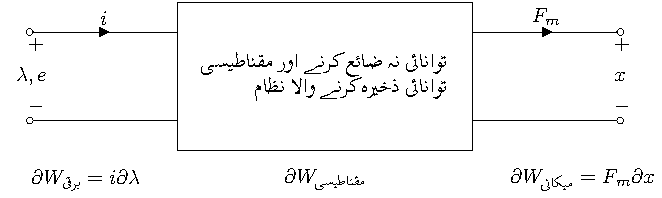
\includegraphics{figEnergyConversionBasicBlockDiagramDetailed}
\caption{توانائی کی شکل تبدیل کرنے والا ایک نظام۔}
\label{شکل_تبادلہ_توانائی_قوت_پیدا_کرتا_آلا_زیادہ_معلومات}
\end{figure}

	کسی بھی تفاعل\حاشیہب{function} \عددیء{z(x,y)} کے لئے ہم لکھ سکتے ہیں
\begin{align}\label{مساوات_تبادلہ_جزوی_تفرق_عمومی_الف}
\partial z(x,y)=\frac{\partial z}{\partial x} \dif x+\frac{\partial z}{\partial y} \dif y
\end{align}
اسی طرح ہم \عددیء{W_m(x,\lambda)} کے لئے لکھ سکتے ہیں۔
\begin{align}\label{مساوات_تبادلہ_جزوی_تفرق_عمومی_ب}
\partial W_m(x,\lambda)=\frac{\partial W_m}{\partial x}\dif x+\frac{\partial W_m}{\partial \lambda}\dif \lambda
\end{align}
اس مساوات اور مساوات \حوالہ{مساوات_برقی_مقناطیسی_تبادلہ_توانائی_کا_طریقہ} سے ہم اخذ کر سکتے ہیں کہ
\begin{align}
F_m(x,\lambda)&=-\left. \frac{\partial W_m(x,\lambda)}{\partial t}\right|_{\lambda_0}\label{مساوات_تبادلہ_توانائی_قوت_برقی_رو}\\
i(x,\lambda)&=\left. \frac{\partial W_m(x,\lambda)}{\partial \lambda}\right|_{x_0}\label{مساوات_تبادلہ_توانائی_سے_رو}
\end{align}
اگر ہم مقناطیسی میدان میں مقناطیسی توانائی \عددیء{W_m(x,\lambda)} معلوم کر سکیں تو مساوات \حوالہ{مساوات_تبادلہ_توانائی_قوت_برقی_رو}  کو استعمال کر کے ہم قوت کا حساب لگا سکتے ہیں۔ ہم اگلے حصہ میں یہی کرتے ہیں۔

\حصہ{تبادلہ توانائی والا ایک لچھے کا نظام}
شکل \حوالہ{شکل_تبادلہ_توانائی_قوت_پیدا_کرتا_آلا}  میں  ایک لچھے کا سادہ نظام دکھایا گیا ہے۔ لچھے میں برقی ضیاع کو بیرونی مزاحمت سے پیش کیا گیا ہے۔ میکانی نظام میں حرکت کرنے والے حصہ کے کمیت کو نظرانداز کیا گیا ہے۔ اگر اس کمیت  کے اثر کا بھی حساب لگانا ہو تو اس کمیت کو ایک بیرونی کمیت تصور کیا جا سکتا ہے۔ اس طرح تبادلہ توانائی کے نظام پر غور کرنا آسان ہو جاتا ہے۔ 

قوت پیدا کرنے والے مشین میں حرکت ناگزیر ہے۔عموماً حرکت تب ممکن ہوتی ہے جب مقناطیسی قالب میں خلاء ہو جو کم اور زیادہ ہو سکے۔  عموماً \عددیء{\Re_a \gg \Re_c} ہوتا ہے۔لہٰذا جب بھی خلائی درز رکنے والی  مقناطیسی دور حل کرنی ہو،  ہم \عددیء{\Re_c} کو نظرانداز کر سکتے ہیں۔ایسا کرنے سے، جیسا مساوات \حوالہ{مساوات_مقناطیسی_ڈور_بہاو_مساوی_دباو_بٹا_ہچکچاہٹ}  میں دیا گیا ہے، ہم  مقناطیسی دباو \عددیء{\tau} اور مقناطیسی بہاو \عددیء{\phi} کو براہ راست متناسب لکھ سکتے ہیں۔ اسی طرح مساوات \حوالہ{مساوات_مقناطیسی_دور_خود_امالہ_تعریف}   کو اب  ہم  یوں لکھ سکتے ہیں
\begin{align}\label{مساوات_تبادلہ_ارتباط_بہاو_اور_امالہ}
\lambda=L(x) i
\end{align}
اس مساوات میں امالہ  کو \عددیء{L(x)} لکھ کر اس بات کی نشاندہی کی گئی ہے کہ یہ صرف اور صرف  شکل \حوالہ{شکل_تبادلہ_توانائی_قوت_پیدا_کرتا_آلا}   میں خلاء کی لمبائی \عددیء{x} پر منحصر ہے۔

شکل \حوالہ{شکل_تبادلہ_توانائی_قوت_پیدا_کرتا_آلا}  میں قوت \عددیء{F_m}  کی سمت میں طے ہونے والا فاصلہ \عددیء{x} ہے۔ یوں  میکانی کام \عددیء{\partial W_{\textup{میکانی}}=F_m \dif x} کے برابر ہو گا جبکہ  \عددیء{\partial W_{\textup{برقی}}=i \dif \lambda}۔ یوں شکل \حوالہ{شکل_تبادلہ_توانائی_قوت_پیدا_کرتا_آلا}   کو مساوات \حوالہ{مساوات_برقی_مقناطیسی_تبادلہ_توانائی_کا_طریقہ}  ظاہر کرتی ہے۔ اگر ہمیں مقناطیسی میدان میں ذخیرہ توانائی \عددیء{W_m} معلوم کرنی ہو تو ہمیں مساوات \حوالہ{مساوات_برقی_مقناطیسی_تبادلہ_توانائی_کا_طریقہ}  کا تکمل\حاشیہب{integral}  لینا ہو گا۔ یعنی
\begin{align}\label{مساوات_تبادلہ_توانائی_تکمل}
\int \partial W_m = \int i(x,\lambda) \dif \lambda-\int F_m(x,\lambda) \dif x
\end{align}
اس تکمل کا حصول شکل \حوالہ{شکل_تبادلہ_توانائی_مقناطیسی_میدان_میں_توانائی}   سے واضح ہو گا۔ابتدائی نقطے پر مقناطیسی نظام کو کوئی برقی توانائی نہیں دی گئی۔ اس لئے اس میں  برقی رو صفر ہے۔ برقی رو صفر ہونے کی وجہ سے  مقناطیسی بہاو اور  ارتباط بہاو بھی صفر ہے۔اسی وجہ سے مقناطیسی میدان میں مقناطیسی توانائی بھی صفر ہے۔یوں  قوت اور حرکت بھی صفر ہے۔ یعنی ابتدائی نقطہ پر
\begin{align*}
i=\phi=\lambda=W_m=F_m=x=0
\end{align*}
ہے۔ابتدائی نقطہ شکل \حوالہ{شکل_تبادلہ_توانائی_مقناطیسی_میدان_میں_توانائی}  میں دکھایا گیا ہے۔ ہم اب لچھے کو برقی توانائی فراہم کرتے ہیں۔ لچھے میں برقی رو رواں ہوتی ہے جس سے قوت اور حرکت پیدا ہوتی ہے۔ ہم آخر کار  اختتامی نقطے پہ پہنچ جاتے ہیں۔اختتامی نقطہ بھی شکل میں دکھایا گیا ہے۔ اس نقطہ پہ \عددیء{\lambda=\lambda_0} اور \عددیء{x=x_0} ہے اور یہاں مقناطیسی میدان میں توانائی \عددیء{W_m(x_0,\lambda_0)} ہے۔ہم ابتدائی نقطہ  سے اختتامی نقطہ  تک پہنچنے کے لئے  برقی توانائی کو یوں بڑھاتے ہیں کہ \عددیء{\lambda} اور \عددیء{x}  شکل \حوالہ{شکل_تبادلہ_توانائی_مقناطیسی_میدان_میں_توانائی}  میں موٹی لکیر سے دکھائے اصل راستے پر رہیں۔لہٰذا ہمیں آخری نقطہ پہ مقناطیسی میدان میں مقناطیسی توانائی \عددیء{W_m(x_0,\lambda_0)} معلوم کرنے کے لئے مساوات \حوالہ{مساوات_تبادلہ_توانائی_تکمل}  کا اصل راستے پہ تکمل کرنا ہو گا۔ ایسا کرنا خاصا مشکل کام ہے۔ بجائے یہ ہم ایک بہتر راستہ اختیار کرتے ہیں۔
\begin{figure}
\centering
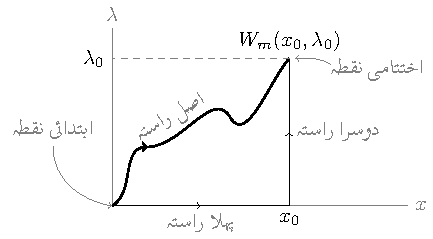
\includegraphics{figEnergyConversionEnergyInMagneticField}
\caption{مقناطیسی میدان میں توانائی۔}
\label{شکل_تبادلہ_توانائی_مقناطیسی_میدان_میں_توانائی}
\end{figure}


ہم اس حقیقت سے فائدہ اٹھاتے ہیں کہ مقناطیسی میدان ایک \اصطلاح{قدامت پسند میدان}\فرہنگ{قدامت پسند میدان}\حاشیہب{conservative field}\فرہنگ{conservative field}   ہے جس کا مطلب ہے کہ مقناطیسی میدان میں مقناطیسی توانائی صرف اور صرف اختتامی نقطہ کے \عددیء{x_0} اور \عددیء{\lambda_0} کی مقدار پر منحصر ہے\حاشیہد{تجاذبی میدان بھی قدامت پسند میدان ہے اسی لئے اگر کمیت \عددیء{m} کو کسی بھی راستے \عددیء{h} کی بلندی تک لے جایا جائے تو اس کی توانائی \عددیء{mgh} ہو گی۔}۔ اس کا مطلب یہ ہے کہ ہم جس راستے سے بھی آخری نقطہ تک پہنچیں ہمیں مقناطیسی میدان میں مقناطیسی توانائی یکساں ملے گی۔ لہٰذا ہم تکمل کرتے وقت شکل  \حوالہ{شکل_تبادلہ_توانائی_مقناطیسی_میدان_میں_توانائی} میں ابتدائی نقطہ سے  پہلے راستے چلتے ہیں اور جب ہم  فاصلہ  \عددیء{x_0} طے کر لیں تو یہاں سے دوسرا راستہ اختیار کر کے اختتامی نقطہ \عددیء{(x_0,\lambda_0)} پہ پہنچتے ہیں۔ لہٰذا ہم مساوات \حوالہ{مساوات_تبادلہ_توانائی_تکمل}   کو اب دو ٹکڑوں میں لکھیں گے، نقطہ \عددیء{(0,0)} سے نقطہ  \عددیء{(x_0,0)} تک اور پھر یہاں سے نقطہ \عددیء{(x_0,\lambda_0)}  تک
\begin{align}\label{مساوات_تبادلہ_توانائی_تکمل_راستہ_دو_ٹکڑے}
\int\limits_{\textup{اصل راستہ}} \partial W_m =\int\limits_{\textup{پہلا راستہ}} \partial W_m +\int\limits_{\textup{دوسرا راستہ}} \partial W_m 
\end{align}
اس مساوات کی دائیں جانب جزو کو باری باری دیکھتے ہیں۔پہلے راستے تکمل کو یوں لکھا جا سکتا ہے۔
\begin{align}\label{مساوات_تبادلہ_توانائی_تکمل_پہلا_راستہ}
\int\limits_{\textup{پہلا راستہ}} \partial W_m =\int_0^0 i(x,0) \dif \lambda-\int_0^{x_0} F_m(x,0) \dif x
\end{align}
	اس  راستے جیسے شکل \حوالہ{شکل_تبادلہ_توانائی_مقناطیسی_میدان_میں_توانائی}  سے ظاہر ہے اگر ہم \عددیء{x=0} سے  \عددیء{x=x_0} تک چلیں تو اس پورے راستے پر \عددیء{\lambda} صفر کے برابر ہی رہتا ہے۔ مساوات \حوالہ{مساوات_تبادلہ_توانائی_تکمل_پہلا_راستہ}  میں اس بات کو برقی رو \عددیء{i(x,0)}  اور قوت \عددیء{F_m(x,0)}  لکھ کر واضح کیا گیا ہے۔ چونکہ \عددیء{\lambda} کے شروع اور آخری مقدار  برابر ہیں لہٰذا اس مساوات میں \عددیء{\int_0^0 i(x,0)\dif \lambda =0} ہے۔

 اگر \عددیء{\lambda=0} ہو تو مقناطیسی بہاو بھی صفر ہو گا۔ مقناطیسی بہاو کے صفر ہونے کا مطلب ہے کہ کوئی مقناطیسی اثر موجود نہیں لہٰذا قوت \عددیء{F_m} بھی صفر ہو گا۔ اور ہم جانتے ہیں کہ صفر کا تکمل صفر ہی ہوتا ہے۔ لہٰذا اس مساوات میں \عددیء{\int_0^{x_0} F_m(x,0)\dif x=0} ہو گا۔ یوں پہلے راستے پر تکمل یعنی مساوات \حوالہ{مساوات_تبادلہ_توانائی_تکمل_پہلا_راستہ}  صفر کے برابر ہے یعنی
\begin{align}
\int\limits_{\textup{پہلا راستہ}} \partial W_m =\int_0^0 i(x,0) \dif \lambda-\int_0^{x_0} F_m(x,0) \dif x=0
\end{align}
اسی طرح مساوات \حوالہ{مساوات_تبادلہ_توانائی_تکمل_راستہ_دو_ٹکڑے} کی دوسرے راستے کے تکمل کے جزو کو یوں لکھا جا سکتا ہے۔
\begin{align}
\int\limits_{\textup{دوسرا راستہ}} \partial W_m =\int_0^{\lambda_0} i(x_0,\lambda) \dif \lambda-\int_{x_0}^{x_0} F_m(x_0,\lambda) \dif x
\end{align}
اس میں ہم دیکھتے ہیں کہ پورے راستے \عددیء{x=x_0} رہتا ہے۔ قوت کا تکمل صفر ہے چونکہ  \عددیء{x} کے  ابتدائی اور اختتامی قیمتیں برابر ہیں۔  یعنی
\begin{align}
\int_{x_0}^{x_0} F_m(x_0,\lambda) \dif x=0
\end{align}
آخر میں رہ گیا برقی رو کا تکمل۔ مساوات \حوالہ{مساوات_تبادلہ_ارتباط_بہاو_اور_امالہ}  کو استعمال کرتے ہوئے
\begin{align}
\int_0^{\lambda_0} i(x_0,\lambda) \dif \lambda=\frac{1}{L(x_0)} \int_0^{\lambda_0} \lambda \dif \lambda=\frac{\lambda_0^2}{2 L(x_0)}
\end{align}
اس طرح ہمیں آخر کار مقناطیسی میدان میں توانائی کی مساوات حاصل ہو گئی۔
\begin{align}
W=\frac{\lambda_0^2}{2 L(x_0)}
\end{align}

اس مساوات کی مدد سے مساوات \حوالہ{مساوات_تبادلہ_توانائی_قوت_برقی_رو}  کے ذریعہ قوت  \عددیء{F_m(x,\lambda)} اور مساوات \حوالہ{مساوات_تبادلہ_توانائی_سے_رو}  کے ذریعہ برقی رو \عددیء{i(x,\lambda)}  کا حساب اب ممکن ہے۔
%
\ابتدا{مثال}\شناخت{مثال_تبادلہ_توانائی_درز_میں_مقناطیسی_توانائی}
شکل \حوالہ{شکل_تبادلہ_توانائی_حرکت_اور_توانائی}  میں حرکت کرنے والا ایک مقناطیسی نظام دکھایا گیا ہے۔ حرکت کرنے والے حصے اور ساکن حصے  کے مابین خلائی درز \عددیء{g} ہے۔ اگر \عددیء{N=500} ،\عددیء{g=\SI{1}{\milli \meter}} ،\عددیء{b=\SI{0.2}{\meter}}، \عددیء{w=\SI{0.4}{\meter}} اور \عددیء{i=\SI{30}{\ampere}} ہوں تو اس خلائی درز میں توانائی \عددیء{W_m} معلوم کریں۔
\begin{figure}
\centering
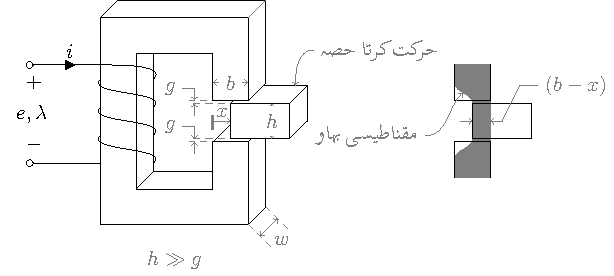
\includegraphics{figEnergyConversionForceOnPlunger}
\caption{حرکت اور توانائی۔}
\label{شکل_تبادلہ_توانائی_حرکت_اور_توانائی}
\end{figure}

حل:
چونکہ \عددیء{h \gg g} ہے لہٰذا مقناطیسی بہاو کا بیشتر حصہ حرکت کرتے حصے سے گزرے گا۔ساکن حصے میں مقناطیسی بہاو خلائی درز کے قریب مڑ کر حرکت کرتے حصے میں سے گزرے گا۔ہمیں معلوم ہے کہ \عددیء{W_m=\tfrac{\lambda^2}{2L}}  اور \عددیء{L=\lambda i} ہیں لہٰذا \عددیء{W_m=\tfrac{1}{2} L i^2} لکھا جا سکتا ہے جہاں \عددیء{L=\tfrac{N^2 \mu_0 A_g}{2 g}} اور \عددیء{A_g=w(b-x)} کے برابر ہیں۔یوں
\begin{align*}
W_m&=\frac{1}{2} \frac{N^2 \mu_0 A_g}{2 g } i^2\\
&=\frac{1}{2} \times \frac{500^2 \times 4 \pi 10^{-7} \times 0.4 (0.2-x)}{2 \times 0.001} \times 30^2\\
&=28278 (0.2-x)
\end{align*}
جاول کے برابر ہے۔
\انتہا{مثال}
%
\ابتدا{مثال}\شناخت{مثال_تبادلہ_توانائی_قوت_کا_حصول_بذریعہ_توانائی_طریقہ}
 شکل \حوالہ{شکل_تبادلہ_توانائی_حرکت_اور_توانائی} میں توانائی کے طریقہ سے قوت \عددیء{F_m} معلوم کریں۔

حل:
	 مساوات \حوالہ{مساوات_تبادلہ_توانائی_قوت_برقی_رو}  کہتا ہے کہ \عددیء{F_m=-\left. \tfrac{\partial W_m(x,\lambda)}{\partial x} \right|_{\lambda_0}} ہے۔اس کا مطلب ہے کہ توانائی کے متغیرہ \عددیء{x} اور \عددیء{\lambda} ہونے چاہئے۔

مثال \حوالہ{مثال_تبادلہ_توانائی_درز_میں_مقناطیسی_توانائی} میں ہم نے توانائی معلوم کی۔البتہ یہ معلوم کرنے  کے لئے ہم نے \عددیء{\lambda} کی  بجائے \عددیء{\lambda=L i} استعمال کیا۔ یوں  توانائی کے متغیرہ  \عددیء{x} اور \عددیء{i} بن گئے ۔  ہم \عددیء{W_m(x,i)=28278 (0.2-x)} کو استعمال نہیں کر سکتے۔ ہمیں \عددیء{W_m(x,\lambda)} چاہئے۔ درست طریقہ یہ ہے
\begin{align*}
W_m(x,\lambda)=\frac{\lambda^2}{2 L}=\frac{\lambda^2}{2 \left(\frac{N^2 \mu_0 A_g}{2 g} \right)}=\frac{ g \lambda^2}{N^2 \mu_0 w (b-x)}
\end{align*}
اب اسے مساوات \حوالہ{مساوات_تبادلہ_توانائی_قوت_برقی_رو} میں استعمال کرتے ہوئے
\begin{align*}
F_m&=-\frac{\partial W_m(x,\lambda)}{\partial x}\\
&=-\frac{g \lambda^2}{N^2 \mu_0 w (b-x)^2}
\end{align*}
تفرق لینے کے بعد \عددیء{\lambda} کی جگہ \عددیء{L i} پُر کیا جا سکتا ہے۔یوں قوت
\begin{align*}
F_m&=-\frac{g L^2 i^2}{N^2 \mu_0 w (b-x)^2}\\
&=-\frac{N^2 \mu_0 w i^2}{4 g}\\
&=\num{-28278}
\end{align*}
نیوٹن حاصل ہوتا ہے۔منفی قوت کا مطلب ہے کہ قوت \عددیء{x} کی اُلٹ جانب ہے یعنی حرکت کرنے والا حصہ اس جانب حرکت کرے گا جس جانب فاصلہ کم ہوتا ہو۔
\انتہا{مثال}
%
\حصہ{توانائی اور کو-توانائی}
	شکل \حوالہ{شکل_تبادلہ_توانائی_کو_توانائی_کی_تعریف}  میں \عددیء{\lambda} اور \عددیء{i} کے مابین گراف دکھایا گیا ہے۔ جیسا آپ دیکھ سکتے ہیں کہ لکیر کے نیچے رقبہ دراصل توانائی ہی ہے۔ اگر ہم اس گراف پر کوئی ایک نقطہ \عددیء{(\lambda,i)} لیں اور اس نکتے سے ایک لکیر نیچے کی طرف اور دوسری لکیر بائیں جانب کھینچے تو ہمیں ایک مستطیل ملتا ہے جس کا رقبہ \عددیء{\lambda i} کے برابر ہو گا۔ اگر اس میں سے ہم توانائی  \عددیء{W_m} منفی کر لیں تو جو مقدار ملتی ہے اس کو کو-توانائی \عددیء{W_m'} کہتے ہیں یعنی
\begin{figure}
\centering
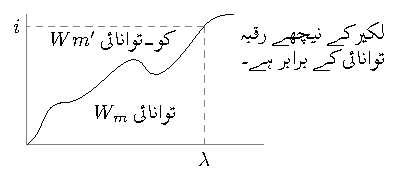
\includegraphics{figEnergyConversionDefiningCoenergy}
\caption{کو-توانائی کی تعریف۔}
\label{شکل_تبادلہ_توانائی_کو_توانائی_کی_تعریف}
\end{figure}

\begin{align}
W_m'=\lambda i -W_m
\end{align}
اس مساوات کے تدریجی تفرق\فرہنگ{تدریجی تفرق}\حاشیہب{partial differential}
\begin{align*}
\partial W_m'&=\partial (\lambda i) -\partial W_m\\
&=\lambda \partial i + i \partial \lambda -\partial W_m
\end{align*}
میں مساوات \حوالہ{مساوات_برقی_مقناطیسی_تبادلہ_توانائی_کا_طریقہ}  کے استعمال سے
\begin{align*}
\partial W_m'&=\lambda \partial i + i \partial \lambda -(i \partial \lambda-F_m \partial x)
\end{align*}
یعنی
\begin{align}\label{مساوات_تبادلہ_کو_توانائی_تعریفی_مساوات}
\partial W_m'&=\lambda \partial i + F_m \partial x
\end{align}
حاصل ہوتا ہے۔

مساوات \حوالہ{مساوات_تبادلہ_جزوی_تفرق_عمومی_الف}  ،\حوالہ{مساوات_تبادلہ_جزوی_تفرق_عمومی_ب} ،\حوالہ{مساوات_تبادلہ_توانائی_قوت_برقی_رو}  اور \حوالہ{مساوات_تبادلہ_توانائی_سے_رو}  کی طرح یہاں بھی کسی بھی تفاعل \عددیء{z(x,y)} کا تدریجی فرق
\begin{align*}
\partial z(x,y)=\frac{\partial z}{\partial x} \dif x+\frac{\partial z}{\partial y} \dif y
\end{align*}
ہے۔یوں ہم  کو-توانائی \عددیء{W_m'(x,i)} کے لئے لکھ سکتے ہیں
\begin{align}
\partial W_m'(x,i)=\frac{\partial W_m'}{\partial x} \dif x+\frac{\partial W_m'}{\partial i} \dif i
\end{align}
اس مساوات کو مساوات \حوالہ{مساوات_تبادلہ_کو_توانائی_تعریفی_مساوات}  کے سات دیکھیں تو  
\begin{align}
\lambda&=\left. \frac{\partial W_m'}{\partial i} \right|_{x_0}\\
\intertext{اور}
F_m&=\left. \frac{\partial W_m'}{\partial x} \right|_{i_0}\label{مساوات_تبادلہ_کوتوانائی_سے_قوت}
\end{align}
حاصل ہوتے ہیں۔قوت معلوم کرنے  کی یہ دوسری مساوات ہے۔ اس مساوات میں کو-توانائی استعمال ہوتی ہے جبکہ مساوات \حوالہ{مساوات_تبادلہ_توانائی_قوت_برقی_رو} میں  توانائی کے ذریعہ قوت  حاصل کی گئی۔

بالکل توانائی کے طریقہ سے ان مساوات کے تکمل سے حاصل ہوتا ہے
\begin{align}
W_m'(i_0,x_0)=\int_{0}^{i_0} \lambda(i,x_0) \dif i
\end{align}
جن نظام میں \عددیء{\lambda} اور \عددیء{i} تغیر راست ہوں اور جنہیں مساوات \حوالہ{مساوات_مقناطیسی_دور_خود_امالہ_تعریف} کے تعلق سے پیش کیا جا سکے ان کے لئے اس مساوات کو مزید یوں حل کیا جا سکتا ہے۔
\begin{align}\label{مساوات_تبادلہ_کوتوانائی_مساوی_امالہ_مربع_رو}
W_m'(i,x)=\int_{0}^{i} L(x) i  \dif i=\frac{L(x) i^2}{2}
\end{align}
کچھ مسائل میں توانائی اور  کچھ میں کو-توانائی کا استعمال زیادہ آسان ہوتا ہے۔
%
\ابتدا{مثال}
شکل \حوالہ{شکل_تبادلہ_توانائی_پیچدار_لچھا}  میں ایک پیچدار لچھا\حاشیہب{spiral coil} دکھایا گیا ہے جس کی محوری لمبائی \عددیء{l}،   رداس \عددیء{r}  اور چکر \عددیء{N}  ہیں۔ایسے پیچدار لچھے کی مقناطیسی بہاو محوری سمت میں لچھے کے اندر ہی رہتی ہے۔ لچھے کے باہر مقناطیسی بہاو کی مقدار قابلِ نظر انداز ہوتی ہے۔یوں لچھے کے اندر محوری لمبائی کی سمت میں میدانی شدت \عددیء{H \approx NI/l} ہوتی ہے۔
\begin{figure}
\centering
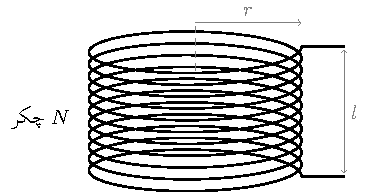
\includegraphics{figEnergyConversionCoil}
\caption{پیچدار لچھا۔}
\label{شکل_تبادلہ_توانائی_پیچدار_لچھا}
\end{figure}

ایسے پیچدار لچھے موصل دھاتوں کو امالی برقی توانائی کے ذریعہ پگھلانے کے لئے استعمال کئے جاتے ہیں۔میں اس طرح کی \عددیء{100}  کلوواٹ سے \عددیء{1500}  کلو واٹ برقی طاقت کی  \عددیء{100} کلوگرام سے  \عددیء{3000} کلوگرام  لوہا پگھلانے کی \اصطلاح{امالی برقی بھٹیاں}\فرہنگ{بھٹی}\حاشیہب{high frequency, induction furnaces} بناتا رہا ہوں جو \عددیء{500} ہرٹز سے  \عددیء{1200} ہرٹز کے درمیاں کام کرتی ہیں۔اس طرح کے پیچدار لچھے میں غیر موصل پیالے میں موصل دھات کے ٹکڑے ڈالے جاتے ہیں اور اس لچھے میں بدلتی رو گزاری جاتی ہے۔دھات میں بھنور نما امالی برقی رو اسے گرم کر کے پگھلا دیتی ہے۔لوہے کو یوں  \عددیء{1650} ڈگری \اصطلاح{ثلسئس}\حاشیہب{Celsius, Centigrade} تک گرم کیا جاتا ہے۔
\begin{itemize}
\item
اس پیچدار لچھے پر معین برقی رو \عددیء{I_0} گزرنے کی صورت میں رداسی سمت میں میکانی دباو یعنی قوت فی مربع رقبہ معلوم کریں۔
\item
میری \عددیء{3000} کلوگرام لوہا پگھلانے کی بھٹی کے پیچدار لچھے کی تفصیل کچھ یوں ہے۔
\begin{align*}
N=11, \quad I_0=\SI{10000}{\ampere}, \quad l=\SI{0.94}{\meter}, \quad r=\SI{0.49}{\meter}
\end{align*}
اس پر رداسی سمت میں میکانی دباو، نیوٹن فی مربع میٹر، میں حاصل کریں۔
\end{itemize}

حل الف:

ہم کو-توانائی کا طریقہ استعمال کرتے ہیں۔
\begin{align*}
L&=\frac{\mu_0 N^2 \pi r^2}{l}\\
W_m'(r,i)&=\frac{L i^2}{2}=\frac{\mu_0 N^2 \pi r^2 I_0^2}{2 l}\\
F&=\frac{\partial W_m'}{\partial r}=\frac{\mu_0 N^2 \pi r I_0^2}{l}
\end{align*}
یہ مثبت قوت رداسی سمت میں باہر کی جانب ہے۔لچھے کی گول سطح  \عددیء{A=2\pi rl} ہے۔یوں میکانی دباو
\begin{align*}
\frac{F}{A}=\frac{\mu_0 N^2 \pi r I_0^2}{2\pi r l^2}=\frac{\mu_0 N^2  I_0^2}{2 l^2}
\end{align*}
ہے۔

حل ب:
\begin{align*}
\frac{F}{A}=\frac{4\pi 10^{-7} \times 11^2 \times 10000^2 }{2 \times 0.94^2}=\SI{8605}{\newton \per \meter \squared}
\end{align*}
\انتہا{مثال}
%
\ابتدا{مثال}
 \عددیء{2000} کلوواٹ سے \عددیء{3000}  کلوواٹ کی لوہا پگھلانے کی بھٹیاں \عددیء{30} ٹن\حاشیہد{ہزار کلوگرام ایک ٹن کے برابر ہوتے ہیں۔} سے \عددیء{70} ٹن لوہا روزانہ پگھلاتی ہیں۔\حاشیہد{یہ میں اپنے تجربے کی بنیاد پر کہہ رہا ہوں۔}اتنا وزن ایک جگہ سے دوسری جگہ منتقل کرنے کی خاطر عموماً برقی مقناطیس استعمال ہوتا ہے۔شکل \حوالہ{شکل_تبادلہ_توانائی_برقی_مقناطیس}-الف میں ایک ایسا ہی برقی مقناطیس دکھایا گیا ہے جس کی تفصیل کچھ یوں ہے۔
\begin{align*}
N=300, \quad A=\SI{0.8}{\meter \squared}, \quad I=\SI{30}{\ampere}
\end{align*}
اگر برقی مقناطیسی اور لوہے کے درمیان اوسط فاصلہ \عددیء{2.5} سنٹی میٹر لیا جائے تو یہ برقی مقناطیسی کتنی کمیت لوہا اٹھا سکتی ہے۔
\begin{figure}
\centering
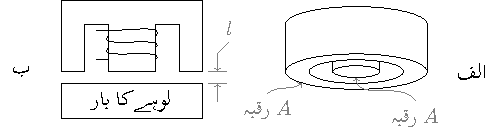
\includegraphics{figEnergyConversionElectroMagnet}
\caption{برقی مقناطیس۔}
\label{شکل_تبادلہ_توانائی_برقی_مقناطیس}
\end{figure}

حل:
\begin{align*}
L&=\frac{\mu_0 N^2 A}{2 l}\\
W_m'(l,i)&=\frac{L i^2}{2}=\frac{\mu_0 N^2 A i^2}{4 l}\\
F&=\frac{\partial W_m}{\partial l}=-\frac{\mu_0 N^2 A i^2}{4 l^2}=-\frac{4\pi 10^{-7} \times 300^2 \times 0.8  \times 30^2}{4 \times 0.0254^2}=\SI{31558}{\newton}
\end{align*}
یوں یہ مقناطیس \عددیء{\tfrac{31558}{9.8}=\SI{3220}{\kilo\gram}} کمیت اٹھا سکتا ہے۔
\انتہا{مثال}
%
\ابتدا{مثال}
مثال \حوالہ{مثال_تبادلہ_توانائی_قوت_کا_حصول_بذریعہ_توانائی_طریقہ} کو کو-توانائی کے طریقہ سے حل کریں۔

حل:
مساوات \حوالہ{مساوات_تبادلہ_کوتوانائی_مساوی_امالہ_مربع_رو}   سے
\begin{align*}
W_m'&=\frac{L(x) i^2}{2}=\frac{N^2 \mu_0 w(b-x) i^2}{4 g}
\end{align*}
اور مساوات \حوالہ{مساوات_تبادلہ_کوتوانائی_سے_قوت}  سے
\begin{align*}
F_m=\frac{\partial W_m}{\partial x}=-\frac{N^2 \mu_0 w i^2}{4 g}=\SI{-28278}{\newton}
\end{align*}
یہ اتنی ہی قوت ہے۔ہونا بھی ایسا ہی چاہئے۔
\انتہا{مثال}
%
\حصہ{زیادہ لچھوں کا مقناطیسی نظام}
ابھی تک صرف ایک لچھے کے نظام کا مطالعہ کیا گیا ہے۔ اس حصہ میں  ایک سے زیادہ لچھوں کے نظام کا مطالعہ کیا جائے گا۔ زیادہ لچھوں کا نظام بھی بالکل ایک لچھے کے نظام کی طرح حل ہوتے ہیں۔
\begin{figure}
\centering
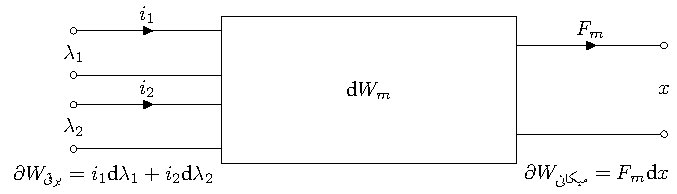
\includegraphics{figEnergyConversionBasicBlockDiagramDetailedTwoCoils}
\caption{ دو لچھوں کا نظام۔}
\label{شکل_تبادلہ_توانائی_دو_لچھوں_کا_نظام}
\end{figure}
%
شکل \حوالہ{شکل_تبادلہ_توانائی_دو_لچھوں_کا_نظام}  میں بائیں جانب ایک لچھے کا برقی رو \عددیء{i_1} اور دوسرے لچھے کا برقی رو \عددیء{i_2} ہے۔ لہٰذا
\begin{align}
\partial W_{\textup{برقی}}&=i_1 \dif \lambda_1+i_2 \dif \lambda_2\\
\partial W_{\textup{برقی}}&=\partial W_{\textup{میکانی}}+\partial W_m\\
i_1 \dif \lambda_1+i_2 \dif \lambda_2&=F_m \dif x+\partial W_m
\end{align}
لکھا جا سکتا ہے جہاں پہلی مساوات کو دوسری میں پُر کرتے ہوئے تیسری مساوات حاصل کی گئی جسے مزید یوں لکھ سکتے ہیں۔
\begin{align}\label{مساوات_تبادلہ_دو_لچھے_الف}
\partial W_m(\lambda_1,\lambda_2,x)=i_1 \dif \lambda_1+i_2 \dif \lambda_2-F_m \dif x
\end{align}
اب بالکل مساوات \حوالہ{مساوات_تبادلہ_جزوی_تفرق_عمومی_الف}   کی طرح
\begin{align}\label{مساوات_تبادلہ_دو_متغیر_تفرق}
\partial W_m(\lambda_1,\lambda_2,x)=\frac{\partial W_m}{\partial \lambda_1} \dif \lambda_1+\frac{\partial W_m}{\partial \lambda_2} \dif \lambda_2+\frac{\partial W_m}{\partial x} \dif x
\end{align}
اس مساوات میں ہم نے دائیں طرف کی جگہ لکھا ہے۔ مساوات \حوالہ{مساوات_تبادلہ_دو_لچھے_الف} اور \حوالہ{مساوات_تبادلہ_دو_متغیر_تفرق} سے حاصل ہوتا ہے
\begin{align}
i_1&=\left. \frac{\partial W_m(\lambda_1,\lambda_2,x)}{\partial \lambda_1} \right|_{\lambda_2,x}\\
i_2&=\left. \frac{\partial W_m(\lambda_1,\lambda_2,x)}{\partial \lambda_2} \right|_{\lambda_1,x}\\
F_m&=\left. \frac{\partial W_m(\lambda_1,\lambda_2,x)}{\partial x} \right|_{\lambda_1,\lambda_2}
\end{align}
یہ مساوات تب استعمال ہو سکتے ہیں جب ہمیں توانائی \عددیء{W_m} معلوم ہو لہٰذا ہم پہلے اسی کو معلوم کرتے ہیں۔

\begin{figure}
\centering
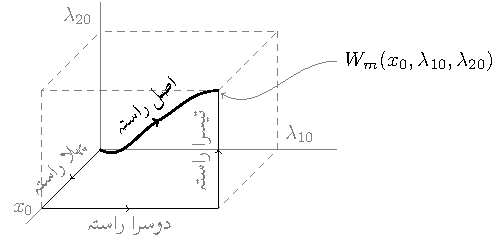
\includegraphics{figEnergyConversionTwoCoilSystemEnergyIntegral}
\caption{دو لچھوں کے نظام میں مقناطیسی میدان میں  توانائی۔}
\label{شکل_تبادلہ_توانائی_دو_لچھوں_کے_توانائی_کا_تکمل}
\end{figure}

شکل \حوالہ{شکل_تبادلہ_توانائی_دو_لچھوں_کا_نظام}  میں دونوں لچھوں کو اس طرح طاقت دی جاتی ہے کہ \عددیء{\lambda_1} اور \عددیء{\lambda_2} آہستہ آہستہ صفر سے بڑھتے ہوئے  \عددیء{\lambda_{1_0}}  اور \عددیء{\lambda_{2_0}} تک پہنچ جاتے ہیں اور سات ہی سات  \عددیء{x} صفر سے تبدیل ہو کر \عددیء{x_0} ہو جاتا ہے۔ اس اصل راستے کو شکل \حوالہ{شکل_تبادلہ_توانائی_دو_لچھوں_کے_توانائی_کا_تکمل}  میں موٹی لکیر  سے ظاہر کیا گیا ہے۔ بالکل مساوات \حوالہ{مساوات_تبادلہ_توانائی_تکمل_راستہ_دو_ٹکڑے}  کی طرح ہم لکھ سکتے ہیں۔
\begin{align}\label{مساوات_تبادلہ_اصل_راستے_پر_تکمل}
\int\limits_{\textup{اصل راستہ}} \partial W_m=\int\limits_{\textup{پہلا راستہ}} \partial W_m+\int\limits_{\textup{دوسرا راستہ}} \partial W_m+\int\limits_{\textup{تیسرا راستہ}} \partial W_m
\end{align}
ہم دائیں جانب کے تکمل کو باری باری حل کرتے ہیں۔
\begin{align}
\int\limits_{\textup{پہلا راستہ}} \partial W_m=\int_{0}^{0} i_1 \dif \lambda_1+\int_{0}^{0} i_2 \dif \lambda_2-\int_0^{x_0} F_m \dif x
\end{align}
اگر تکمل کے ابتدائی  اور اختتامی  نقطے ایک ہی ہوں  تو  تکمل صفر کے برابر ہوتا ہے لہٰذا
\begin{align}
\int_{0}^{0} i_1 \dif \lambda_1=\int_{0}^{0} i_2 \dif \lambda_2=0
\end{align}
ہوں گے۔پہلے راستے \عددیء{\lambda_1} اور \عددیء{\lambda_2} دونوں صفر ہیں۔ اس کا مطلب ہے کہ دونوں لچھوں میں برقی رو صفر ہے، لہٰذا مقناطیسی بہاو کی غیر موجودگی میں قوت \عددیء{F_m=0} ہو گا  
اور صفر کا تکمل صفر ہی ہوتا ہے یعنی
\begin{align}
\int_0^{x_0} F_m \dif x=\int_0^{x_0} 0 \dif x=0
\end{align}
اس طرح
\begin{align}\label{مساوات_تبادلہ_پہلا_راستہ_جزو}
\int\limits_{\textup{پہلا راستہ}} \partial W_m=0
\end{align}
حاصل ہوتا ہے۔دوسرے راستے پر
\begin{align}
\int\limits_{\textup{دوسرا راستہ}} \partial W_m=\int_{0}^{\lambda_{1_0}} i_1 \dif \lambda_1+\int_{0}^{0} i_2 \dif \lambda_2-\int_{x_0}^{x_0} F_m \dif x
\end{align}
جیسا پہلے ذکر کیا گیا کہ اگر تکمل کے ابتدائی اور اختتامی  نقطے ایک ہی ہوں  تو  تکمل صفر کے برابر ہوتا ہے لہٰذا
\begin{align}
\int_{0}^{0} i_2 \dif \lambda_2=\int_{x_0}^{x_0} F_m \dif x=0
\end{align}
ہوں گے جس سے
\begin{align}\label{مساوات_تبادلہ_دوسرا_راستہ_توانائی}
\int\limits_{\textup{دوسرا راستہ}} \partial W_m=\int_{0}^{\lambda_{1_0}} i_1 \dif \lambda_1
\end{align}
رہ جاتا ہے۔یہاں ہمیں مساوات \حوالہ{مساوات_مقناطیسی_دور_ارتباط_دو_لچھے} ، \حوالہ{مساوات_مقناطیسی_دور_دوسرے_لچھے_کی_ارتباط}  اور \حوالہ{مساوات_مقناطیسی_دور_مشترکہ_امالہ_یکساں}   کی ضرورت پڑتی ہے۔ یہ تین مساوات مندرجہ ذیل ہیں
\begin{align}
\lambda_1&=L_{11} i_1+L_{12} i_2\\
\lambda_2&=L_{21} i_1+L_{22} i_2\\
L_{12}&=L_{21}  
\end{align}
ان مساواتوں کو ہم \عددیء{i_1}  اور \عددیء{i_2} کے لئے حل کریں تو حاصل ہوتا ہے۔
\begin{align}
i_1&=\frac{L_{22} \lambda_1-L_{12} \lambda_2}{D} \label{مساوات_تبادلہ_رو_نمبر_ایک}\\
i_2&=\frac{L_{11} \lambda_2-L_{21} \lambda_1}{D}
\end{align}
جہاں
\begin{align}
D=L_{11}L_{22}-L_{12}L_{21}
\end{align}
کے برابر ہے۔اب ہم مساوات  \حوالہ{مساوات_تبادلہ_دوسرا_راستہ_توانائی} میں مساوات \حوالہ{مساوات_تبادلہ_رو_نمبر_ایک}  پُر کرتے ہیں۔ چونکہ دوسرے راستے پہ  \عددیء{\lambda_2} صفر ہے لہٰذا
\begin{align}
\int_0^{\lambda_{1_0}} \left( \frac{L_{22} \lambda_1-L_{12} \lambda_2}{D}\right) \dif \lambda_1=\frac{L_{22}}{D}\int_0^{\lambda_{1_0}} \lambda_1 \dif \lambda_1=\frac{L_{22}\lambda_{1_0}^2}{2D}
\end{align}
کے برابر ہے۔یوں
\begin{align}\label{مساوات_تبادلہ_دوسرہ_راستہ_جزو}
\int\limits_{\textup{دوسرا راستہ}} \partial W_m=\frac{L_{22}\lambda_{1_0}^2}{2D}
\end{align}
حاصل ہوتا ہے۔

اسی طرح تیسرے راستے پر 
\begin{align}
\int\limits_{\textup{تیسرا راستہ}} \partial W_m=\int_{\lambda_{1_0}}^{\lambda_{1_0}} i_1 \dif \lambda_1+\int_{0}^{\lambda_{2_0}} i_2 \dif \lambda_2-\int_{x_0}^{x_0} F_m \dif x
\end{align}
جیسا پہلے ذکر کیا گیا کہ اگر تکمل کے ابتدائی اور اختتامی  نقطے ایک ہی ہوں  تو  تکمل صفر کے برابر ہوتا ہے لہٰذا
\begin{align}
\int_{\lambda_{1_0}}^{\lambda_{1_0}} i_1 \dif \lambda_1=\int_{x_0}^{x_0} F_m \dif x=0
\end{align}
ہوں گے اور بقایا حصے میں \عددیء{i_2} پُر کرتے ہوئے
\begin{gather}
\begin{aligned}
\int_{0}^{\lambda_{2_0}} i_2 \dif \lambda_2&=\int_{0}^{\lambda_{2_0}} \left(\frac{L_{11} \lambda_2-L_{21} \lambda_1}{D} \right) \dif \lambda_2\\
&=\frac{L_{11} \lambda_{2_0}}{2D}-\frac{L_{21}\lambda_{10} \lambda_{20}}{D}
\end{aligned}
\end{gather}
حاصل ہوتا ہے جس سے
\begin{align}\label{مساوات_تبادلہ_تیسرہ_راستہ_جزو}
\int\limits_{\textup{تیسرا راستہ}} \partial W_m=\frac{L_{11} \lambda_{2_0}^2}{2D}-\frac{L_{21}\lambda_{1_0} \lambda_{2_0}}{D}
\end{align}
ملتا ہے۔

مساوات \حوالہ{مساوات_تبادلہ_پہلا_راستہ_جزو} ،\حوالہ{مساوات_تبادلہ_دوسرہ_راستہ_جزو}  اور \حوالہ{مساوات_تبادلہ_تیسرہ_راستہ_جزو}   کو جمع کر کے مساوات \حوالہ{مساوات_تبادلہ_اصل_راستے_پر_تکمل}   کا حل ملتا ہے۔
\begin{align}\label{مساوات_تبادلہ_اصل_راستے_تکمل_کا_جواب}
\int \partial W_m=\frac{L_{22} \lambda_{1_0}^2}{2D}+\frac{L_{11} \lambda_{2_0}^2}{2D}-\frac{L_{21}\lambda_{1_0} \lambda_{2_0}}{D}
\end{align}

اسی طرح اگر ہم کو-توانائی سے حل کرتے تو
\begin{align}
\partial W_m'(x,i_1,i_2)=\lambda_1 \dif i_1+\lambda_2 \dif i_2+F_m \dif x
\end{align}
جہاں
\begin{align}
\lambda_1&=\left. \frac{\partial W_m'(x,i_1,i_2)}{\partial i_1} \right|_{x,i_2}\\
\lambda_2&=\left. \frac{\partial W_m'(x,i_1,i_2)}{\partial i_2} \right|_{x,i_1}\\
F_m&=\left. \frac{\partial W_m'(x,i_1,i_2)}{\partial x} \right|_{i_1,i_2}
\end{align}
اسی طرح مساوات \حوالہ{مساوات_تبادلہ_اصل_راستے_تکمل_کا_جواب}  کی جگہ کو-توانائی کے لئے حاصل ہوتا ہے
\begin{align}
W_m'(x,i_1,i_2)=\frac{1}{2}L_{11}(x) i_1^2+\frac{1}{2} L_{22}(x) i_2^2+L_{12}(x)i_1 i_2
\end{align}
جس سے قوت کی مساوات
\begin{align}
F_m=\frac{i_1^2}{2} \frac{\dif L_{11}(x)}{\dif x}+\frac{i_2^2}{2}\frac{\dif L_{22}(x)}{\dif x}+i_1 i_2 \frac{\dif L_{12}(x)}{\dif x}
\end{align}
حاصل ہوتی ہے۔
%
\ابتدا{مثال}
شکل \حوالہ{شکل_تبادلہ_توانائی_دو_لچھوں_کا_نظام}  میں میکانی کام کو \عددیء{\partial W_{\textup{میکانی}}=T_m \dif \theta}  لکھ کر توانائی کے طریقہ سے حل کریں۔

حل:
\begin{align*}
\partial W_{\textup{برقی}}&=i_1 \dif \lambda_1+i_2 \dif \lambda_2
\end{align*}
اور \عددیء{\partial W_{\textup{میکانی}}=T_m \dif \theta} کو
\begin{align*}
\partial W_{\textup{برقی}}&=\partial W_{\textup{میکانی}}+\partial W_m
\end{align*}
میں پُر کرنے سے
\begin{align}\label{مساوات_تبادلہ_مروڑ_الف}
\partial W_m=i_1 \dif \lambda_1+i_2 \dif \lambda_2-T_m\dif \theta
\end{align}
حاصل ہوتا ہے۔\عددیء{W_m} کے جزوی تفرق
\begin{align*}
\partial W_m(\lambda_1,\lambda_2,\theta)=\frac{\partial W_m}{\partial \lambda_1}\dif \lambda_1+\frac{\partial W_m}{\partial \lambda_2}\dif \lambda_2+\frac{\partial W_m}{\partial \theta}\dif \theta
\end{align*}
کا مساوات \حوالہ{مساوات_تبادلہ_مروڑ_الف} کے ساتھ موازنہ کرنے سے
\begin{align}
i_1&=\left. \frac{\partial W_m(\lambda_1,\lambda_2,\theta)}{\partial \lambda_1} \right|_{\lambda_2,\theta}\\
i_2&=\left. \frac{\partial W_m(\lambda_1,\lambda_2,\theta)}{\partial \lambda_2} \right|_{\lambda_1,\theta}\\
T_m&=-\left. \frac{\partial W_m(\lambda_1,\lambda_2,\theta)}{\partial \theta} \right|_{\lambda_1,\lambda_2}
\end{align}
حاصل ہوتے ہیں۔ان مساوات کا آخری جزو بالکل مساوات \حوالہ{مساوات_تبادلہ_دو_لچھے_الف}  کی طرح ہے۔اس کو حل کرنے کا ایک ایک قدم بالکل مساوات \حوالہ{مساوات_تبادلہ_دو_لچھے_الف} کو حل کرنے کی طرح ہو گا بس فاصلہ \عددیء{x} کی جگہ زاویہ \عددیء{\theta} آئے گا۔یوں جواب میں میدانی توانائی کے متغیرات  \عددیء{\lambda_1,\lambda_2,\theta} ہوں گے یعنی۔
\begin{align}\label{مساوات_گھومتے_مشین_توانائی_بذریعہ_تکمل}
W_m(\lambda_{1_0},\lambda_{2_0},\theta_0)=\int W_m=\frac{L_{22} \lambda_{1_0}^2}{2D}+\frac{L_{11} \lambda_{2_0}^2}{2D}-\frac{L_{21} \lambda_{1_0} \lambda_{2_0}}{D}
\end{align}
اسی طرح کو-توانائی کے لئے جواب یہ ہے
\begin{align}
\partial W_m'(i_1,i_2,\theta)=\lambda_1 \dif i_1+\lambda_2 \dif i_2+T_m \dif \theta
\end{align}
%
\begin{gather}
\begin{aligned}\label{مساوات_تبادلہ_کوتوانائی_سے_مروڑ}
\lambda_1&=\left.\frac{\partial W_m'(i_1,i_2,\theta)}{\partial i_1} \right|_{i_2,\theta}\\
\lambda_2&=\left.\frac{\partial W_m'(i_1,i_2,\theta)}{\partial i_2} \right|_{i_1,\theta}\\
T_m&=\left.\frac{\partial W_m'(i_1,i_2,\theta)}{\partial \theta} \right|_{i_1,i_2}
\end{aligned}
\end{gather}
جہاں
\begin{align}\label{مساوات_تبادلہ_کوتوانائی_از_خود}
W_m'(i_1,i_2,\theta)=\frac{1}{2} L_{11} i_1^2+\frac{1}{2} L_{22} i_2^2+L_{12} i_1 i_2
\end{align}
ہے۔
\انتہا{مثال}
%
\ابتدا{مثال}
شکل \حوالہ{شکل_تبادلہ_توانائی_دو_لچھوں_میں_مروڑ}  میں دو لچھوں کا نظام دکھایا گیا ہے۔اس نظام کا ایک حصہ ساکن رہتا ہے اور دوسرا گھوم سکتا ہے۔افقی لکیر سے گھڑی کی اُلٹی جانب زاویہ \عددیء{\theta}  ناپا جاتا ہے۔لچھوں کی خود امالہ اور مشترکہ امالہ مندرجہ ذیل ہیں۔
\begin{align*}
L_{11}&=20+30\cos 2 \theta\\
L_{22}&=\left(20+30\cos 2\theta \right) \times 10^{-3}\\
L_{12}&=0.15 \cos \theta
\end{align*}
 برقی رو  \عددیء{i_1=\SI{0.02}{\ampere},i_2=\SI{5}{\ampere}} پر قوت مروڑ \عددیء{T_m} معلوم کریں۔
\begin{figure}
\centering
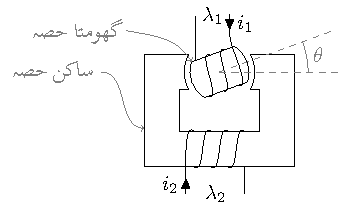
\includegraphics{figEnergyConversionShowingRotor}
\caption{دو لچھوں کے نظام میں قوت مروڑ۔}
\label{شکل_تبادلہ_توانائی_دو_لچھوں_میں_مروڑ}
\end{figure}

حل:مساوات \حوالہ{مساوات_تبادلہ_کوتوانائی_از_خود} سے کو-توانائی حاصل ہوتی ہے اور مساوات \حوالہ{مساوات_تبادلہ_کوتوانائی_سے_مروڑ}  کے آخری جزو سے قوت مروڑ یعنی
\begin{align*}
T_m=\frac{\partial W_m'}{\partial \theta}&=-30 i_1^2 \sin 2 \theta-30\times 10^{-3} i_2^2 \sin 2 \theta -0.15 i_1 i_2 \sin \theta\\
&=-0.012 \sin 2 \theta-0.75 \sin 2 \theta-0.015 \sin \theta\\
&=-0.762 \sin 2 \theta-0.015 \sin \theta
\end{align*}
قوت مروڑ منفی ہونے کا مطلب ہے کہ یہ زاویہ کی اُلٹ سمت میں ہے۔یوں اگر آپ زاویہ بڑھائیں گے تو یہ نظام اسے کم کرنے کی جانب قوت مروڑ پیدا کرے گا اور اگر آپ زاویہ کم کرنے کی کوشش کریں تو یہ زاویہ بڑھانے کی جانب قوت مروڑ پیدا کرے گا۔سادہ زبان میں گھومتا حصہ اُفقی لکیر پر رہنے کی کوشش کرے گا۔
\انتہا{مثال}
